\chapter{Experimental Setup}
\label{chap:setup}

To test the performance of the pipelines in an ideal setup and have a known reference to compare to, the experiments will be performed first using artificially generated data. Whenever generated sonar data is used, the frames come from the same source image that represents the seabed.

\begin{figure}[H]
  \centering
  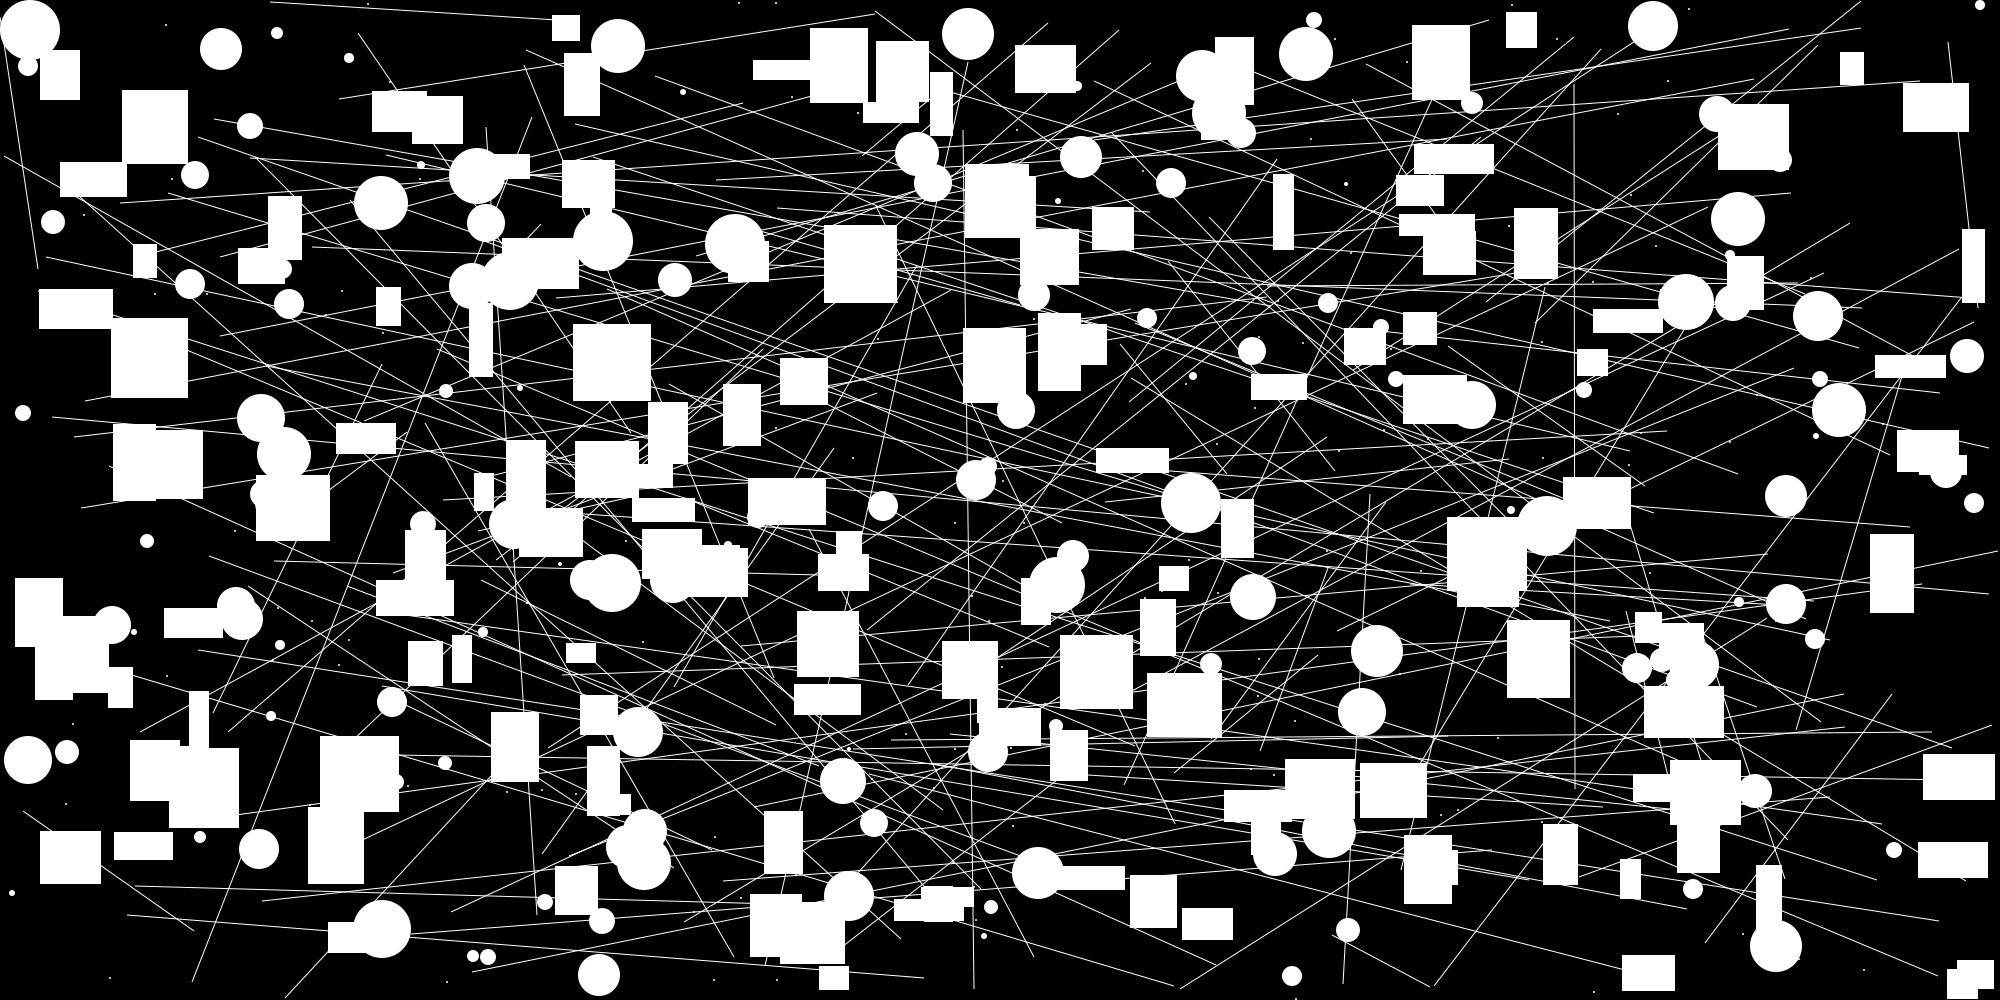
\includegraphics[width=.7\textwidth]{figures/setup/test-reference.png}
  \caption[Source image for fake data]{Artificially generated image used as reference for test sets}
  \label{fig:test_reference}
\end{figure}


Tests using real data use recordings from this area in Trondheim:
\begin{figure}[H]
  \centering
  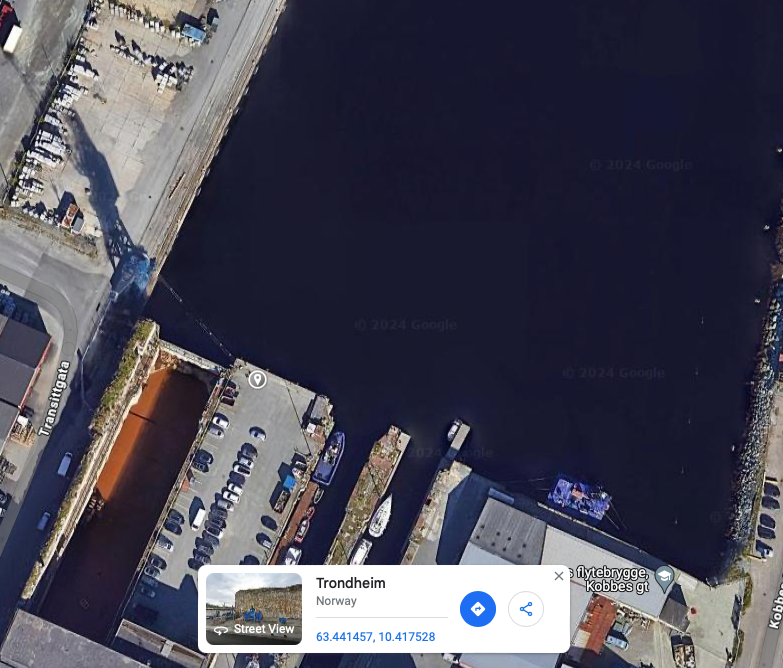
\includegraphics[width=.7\textwidth]{figures/setup/Map.png}
  \caption{Trondheim Harbor testing site: 63.441457, 10.417528}
\end{figure}


To test rotation and translation, three sets of artificial data have been generated:

\begin{enumerate}
    \item Rotation: between each frame there's a rotation of 1º.
    \item Translation: performing a horizontal translation of 10px at every step .
    \item Rotation \& Translation: focusing on the rotation aspect as it's estimation may be affected on distant frames.
\end{enumerate}


As it is interesting to see how the pipelines estimate rotations and translations on distant frames, the test will be repeated skipping 0, 1, 4, and 9 frames in between. This means that for rotations, we would expect to see 1º, 5º, and 10º estimated on the "fake" data, respectively. 

Finally, the pipelines will be tested on real data captured through the \acrshort{rov}. Using the \acrshort{rov}'s DVL data as "ground truth", we can evaluate the accuracy of the measurements. The specs of the sonar used for these tests are the following:


\begin{table}
    \centering
    \begin{tabular}{|c|c|}
        \hline
        \textbf{Parameter} & \textbf{Spec} \\ \hline
        Operating Frequency & 1.2MHz / 2.1MHz \\ \hline
        Range (Maximum) & 40m / 10m \\ \hline
        Range (Minimum) & 0.1m \\ \hline
        Range Resolution & 2.5mm / 2.5mm \\ \hline
        Update Rate (Max.) & 40Hz \\ \hline
        Horizontal Aperture & 130° / 60° \\ \hline
        Vertical Aperture & 20° / 12° \\ \hline
        Number of Beams (Max.) & 512 \\ \hline
        Angular Resolution & 0.6° / 0.4° \\ \hline
        Beam Separation & 0.25° / 0.16° \\ \hline
    \end{tabular}
    \caption{\acrlong{bsosonar} Specs}
    \label{tab:sonar_specs}
\end{table}

The update rate was fixed through sonar settings to be 10Hz. The mentioned 40Hz can only be achieved on very small ranges. 


\begin{table}[H]
    \centering
    \begin{tabular}{|c|c|}
        \hline
        \textbf{Parameter} & \textbf{Spec} \\ \hline
        Ingress protection & IPX8 \\ \hline
        Dimensions & 485 x 257 x 354 mm (LxWxH) \\ \hline
        Weight in air & 8.6 kg (with salt water ballast) \\ \hline
        Buoyancy material & HCP 30 Polymer Foam \\ \hline
        Maximum rated depth & 305 m \\ \hline
        Forward speed at normal use & 1.5 m/s (3 knots) \\ \hline
        Thrusters & 4 x 350 W \\ \hline
        Run time at normal use & 5 hours on High Capacity Battery \\ \hline
        Operating temperature & -10 to +50 °C \\ \hline
    \end{tabular}
    \caption{Blueye X3 \acrshort{rov} Specs}
    \label{tab:drone_specs}
\end{table}

All testing of the pipelines themselves was performed on a MacBook Pro with an M1 Pro processor and 16GB of RAM.

